%==============================================================

\section{Big Data Framework Spark}\label{bds1}

After the features are extracted, the next step is to load the feature files into the HDFS.
All feature files of the same type get merged into one large file. For the about 114000 songs these feature files sum up to about 11.2 GB (see figure \ref{filesize}). 

\begin{figure}[htbp]
	\centering
	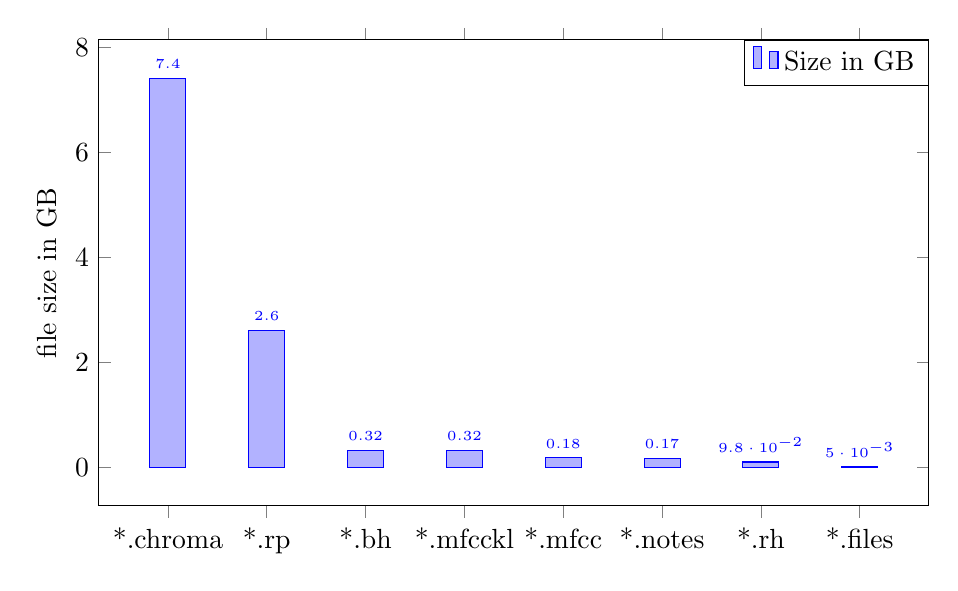
\begin{tikzpicture}
		\begin{axis}[
		    width=\textwidth,height=75mm,% <- added
		    x tick label style={/pgf/number format/1000 sep=},
      		xticklabels={ ,  , *.chroma, *.rp, *.bh, *.mfcckl, *.mfcc, *.notes, *.rh, *.files}, 
		    ylabel=file size in GB,
		    %enlargelimits=0.05,% <- commented, default is .1
		    legend style={
		      at={(1,1)},
		      anchor=north east,% <- changed
		      %legend columns=-1% <- commented
		    },
		    nodes near coords,
		    every node near coord/.append style={font=\tiny},
		    %nodes near coords align={vertical},% <- commented, default
		    ybar=0pt,%<- changed
		    bar width=13pt% <- added
		  ]
		  \addplot
		    coordinates {(1,7.400) (2,2.600) (3,0.324) (4,0.324) (5,0.177) (6,0.174) (7,0.098) (8,0.005)};
		  \legend{Size in GB}
		\end{axis}
	\end{tikzpicture}
	\caption{File sizes}
	\label{filesize}
\end{figure}

\noindent Large streaming platforms like Spotify give access to about 30 million songs in their databases. At this scale, the feature files would be approximately sum up to about 3 TB.\\

\subsubsection{underlying hardware}

The first tests with Spark were performed on a single PC with 4 CPU cores (8 with HT) (Intel Core i7-3610QM CPU, 2.30GHz × 4) running Spark 2.4.0.\\ The cluster test were performed on the ARA- Cluster, that offers 16 compute-nodes with 32 CPU-cores (Dual Socket, 2 x Intel Xeon "Scalable" 6140, 2.30 GHz x 18) per node (72 with HT) and 192GB of RAM. The cluster was running an older version of Spark (1.6.0)\\

\subsection{Data preprocessing}

The features are stored in text files as described in chapter \ref{sumfeat}. Due to the fact that the features were extracted in parallel and in batches of only a few songs, each of the feature files only contain the features of a small number of songs. Because many small files are inefficient to process with Spark \cite[p. 153]{sparkbook1} all files containing the same feature type are merged to one large file, before being loaded into the HDFS. By loading larger files into the HDFS, the partitioning into data blocks is performed according to the standard parameters of the HDFS (e.g. 128 MB partitions). Additional repartitioning on the cluster is later performed with Spark by using the \textit{rdd.repartition(repartition\_count)} command. 
Finally to work with the features a few transformations have to be performed on the data. For example the extracted note values are stored as lists of numbers, each representing a certain note. To compare these using the Levenshtein distance, these lists are converted into strings. 

\begin{pythonCode}[frame=single,label={lst:prep1},caption={notes preprocessing},captionpos=b]
chroma = sc.textFile("features/out[0-9]*.notes").repartition(repartition_count)
chroma = chroma.map(lambda x: x.split(';'))
chroma = chroma.map(lambda x: (x[0], x[1], x[2], x[3].replace("0",'A').replace("1",'B').replace("2",'C').replace("3",'D').replace("4",'E').replace("5",'F').replace("6",'G').replace("7",'H').replace("8",'I').replace("9",'J').replace("10",'K').replace("11",'L'))).map(lambda x: (x[0], x[1], x[2], x[3].replace(',','').replace(' ','')))
df = spark.createDataFrame(chroma, ["id", "key", "scale", "notes"])
\end{pythonCode}

\noindent All the other features are stored as lists of floats and have to be converted to vectors. The Spark ML library and the older MLlib library offer sparse and dense vectors as a data type. The only features that contain a lot of zeros are the beat histograms. Compared to other features like the chromagram they are relatively small (with a length of 200 values) so all lists are converted by calling \lstinline{Vectors.dense(l)}. An example is given for the rhythm pattern features in code snippet \ref{lst:rpp}.

\begin{pythonCode}[frame=single,label={lst:rpp},caption={rp preprocessing},captionpos=b]
from pyspark.mllib.linalg import Vectors
list_to_vector_udf = udf(lambda l: Vectors.dense(l), VectorUDT())
rp = sc.textFile("features[0-9]*/out[0-9]*.rp").repartition(repartition_count)
rp = rp.map(lambda x: x.split(","))
kv_rp = rp.map(lambda x: (x[0].replace(";","").replace(".","").replace(",","").replace(" ",""), list(x[1:])))
rp_df = spark.createDataFrame(kv_rp, ["id", "rp"])
rp_df = rp_df.select(rp_df["id"],list_to_vector_udf(rp_df["rp"]).alias("rp"))
\end{pythonCode}

\noindent The data is read out of the HDFS into an RDD and repartitioned with \lstinline{sc.textFile("name.txt")} and repartitioned. The repartitioning is optional but improves the overall performance (see \ref{sparkperf}). After the pre-processing steps are performed the RDD is converted into a Spark SQL DataFrame by calling \lstinline{spark.createDataFrame()} to ease up the access to the data and improve the code readability. The features can then be accesses via column names instead of the RDD indices. A performance analysis of DataFrames vs. RDDs is also given in section \ref{sparkperf}

\subsection{Distance Computation}

After the data preparation, the similarities between songs can be calculated. 

\subsubsection{Euclidean Distance}

\begin{pythonCode}[frame=single,label={lst:euc},caption={euclidean distance},captionpos=b]
from scipy.spatial import distance
distance_udf = F.udf(lambda x: float(distance.euclidean(x, comparator_value)), FloatType())
result = df_vec.withColumn('distances', distance_udf(F.col('features')))
result = result.select("id", "distances").orderBy('distances', ascending=True)
result = result.rdd.flatMap(list).collect()
\end{pythonCode}

\noindent\textit{\textbf{Explain usage of user defined function udf\\}}
\ \\
\noindent\textit{\textbf{Used with BH, RH, BP AND MFCC\\}}
\ \\
\noindent\textit{\textbf{super versatile AND very fast\\}}
\ \\
\noindent\textit{\textbf{insert analysis of performance\\}}

\subsubsection{Bucketed Random Projection}

Due to the fact that the ARA cluster is running with PySpark version 1.6.0, the Bucketed Random Projection (BRP) Algorithm could only be tested on the single node test platform. 

\begin{pythonCode}[frame=single,label={lst:brp},caption={bucketed random projection},captionpos=b]
from pyspark.ml.feature import BucketedRandomProjectionLSH
#...
brp = BucketedRandomProjectionLSH(inputCol="features", outputCol="hashes", seed=12345, bucketLength=25.0)
model = brp.fit(df_vec)
comparator_value = Vectors.dense(comparator[0])
result = model.approxNearestNeighbors(df_vec, comparator_value, df_vec.count()).collect()
rf = spark.createDataFrame(result)
result = rf.select("id", "distCol").rdd.flatMap(list).collect()
\end{pythonCode}

\noindent\textit{\textbf{Usable as a substitute for euclidean UDF\\}}
\ \\
\noindent\textit{\textbf{Is it faster than the UDF tho? - performance test\\}}

\subsubsection{Cross-correlation}

\textit{\textbf{2 Versions explained - with additional key shift and without}}
\begin{pythonCode}[frame=single,label={lst:corr},caption={cross-correlation},captionpos=b]
def cross_correlate(chroma1, chroma2):
    corr = sp.signal.correlate2d(chroma1, chroma2, mode='full')
    #transposed_chroma = transposed_chroma / (min(length1, length2))
    index = np.where(transposed_chroma == np.amax(transposed_chroma))
    index = int(index[0])
    mean_line = transposed_chroma[index]
    sos = sp.signal.butter(1, 0.1, 'high', analog=False, output='sos')
    mean_line = sp.signal.sosfilt(sos, mean_line)
    return np.max(mean_line)
#...
distance_udf = F.udf(lambda x: float(cross_correlate(x, comparator_value)), DoubleType())
result = df_vec.withColumn('distances', distance_udf(F.col('chroma')))
result = result.select("id", "distances").orderBy('distances', ascending=False)
result = result.rdd.flatMap(list).collect()
\end{pythonCode}

\noindent\textbf{\textit{Memory intense - had to alter spark-defaults.conf\\}}
\textit{spark.driver.memory             6g\\
spark.executor.memory           2g\\
}
\noindent\textbf{\textit{Insert graphics of calculation time with and without correlation\\}}
\ \\
\noindent\textbf{\textit{Differences in the results to the original paper can be explained with the different underlying beat tracking, different filter parameters and a few improvements that are left out as mentioned in \ref{chromafeat}}\cite{cover802}}

\subsubsection{Kullback-Leibler Divergence}

\begin{pythonCode}[frame=single,label={lst:kl},caption={kullback leibler},captionpos=b]
def symmetric_kullback_leibler(vec1, vec2):
	#preprocessing: splitting vec1 and vec2 into mean1, mean2, cov1 and cov2
    d = 13
    div = 0.25 * (np.trace(cov1 * np.linalg.inv(cov2)) + np.trace(cov2 * np.linalg.inv(cov1)) + np.trace( (np.linalg.inv(cov1) + np.linalg.inv(cov2)) * (mean1 - mean2)**2) - 2*d)
    return div
distance_udf = F.udf(lambda x: float(symmetric_kullback_leibler(x, comparator_value)), DoubleType())
result = df_vec.withColumn('distances', distance_udf(F.col('features')))
result = result.select("id", "distances").orderBy('distances', ascending=True)
result = result.rdd.flatMap(list).collect()
\end{pythonCode}

\noindent\textbf{\textit{Differences in the results to the original musly tool can be explained due to the choice of only 13 MFCC bands in this thesis compared to the 25 bands in musly}\cite{musly1}}

\subsubsection{Jensen-Shannon Divergence}

\begin{pythonCode}[frame=single,label={lst:js},caption={jensen shannon},captionpos=b]
def jensen_shannon(vec1, vec2):
	#preprocessing: splitting vec1 and vec2 into mean1, mean2, cov1 and cov2
    mean_m = 0.5 * (mean1 + mean2)
    cov_m = 0.5 * (cov1 + mean1 * np.transpose(mean1)) + 0.5 * (cov2 + mean2 * np.transpose(mean2)) - (mean_m * np.transpose(mean_m))
    div = 0.5 * np.log(np.linalg.det(cov_m)) - 0.25 * np.log(np.linalg.det(cov1)) - 0.25 * np.log(np.linalg.det(cov2))  
    if np.isnan(div):
        div = np.inf
    return div
distance_udf = F.udf(lambda x: float(jensen_shannon(x, comparator_value)), DoubleType())
result = df_vec.withColumn('distances', distance_udf(F.col('features')))
result = result.select("id", "distances").orderBy('distances', ascending=True)
result = result.rdd.flatMap(list).collect()
\end{pythonCode}

\noindent\textbf{\textit{Problem mit den "skyrocketing determinanten" -> Lösung: cholesky zerlegung, geht nicht - nicht positiv definit, Lösung 2 nutzen von SKL aber noch rechenintensiver!}\cite[p.45]{schnitzer1}}

\subsubsection{Levenshtein distance}

\begin{pythonCode}[frame=single,label={lst:lev},caption={levenshtein},captionpos=b]
def get_neighbors_notes(song):
    filterDF = df.filter(df.id == song)
    filterDF.first()
    comparator_value = filterDF.collect()[0][3] 
    print comparator_value
    df_merged = df.withColumn("compare", lit(comparator_value))
    df_levenshtein = df_merged.withColumn("word1_word2_levenshtein", levenshtein(col("notes"), col("compare")))
    df_levenshtein.sort(col("word1_word2_levenshtein").asc()).show()
\end{pythonCode}

\subsubsection{Combining different measurements}

\noindent\textit{\textbf{weighted arithmetic mean of different distance measurements - there has to be some kind of scaling\\}}

\begin{equation} \label{eq:distance}
dist = \frac{\sum_{m = 0}^{M - 1}{w_m \cdot d_m}}{\sum_{m = 0}^{M - 1}{w_m}}
\end{equation}

\noindent\textit{\textbf{statistic prescaling to have mean = 0.5 and variance 0.5?\\}}


\subsection{performance}\label{sparkperf}

\subsubsection{Cluster configuration and data file size}

\begin{pythonCode}[frame=single,label={lst:clust},caption={cluster setup},captionpos=b]
confCluster = SparkConf().setAppName("MusicSimilarity Cluster")
confCluster.set("spark.driver.memory", "64g")
confCluster.set("spark.executor.memory", "64g")
confCluster.set("spark.driver.memoryOverhead", "32g")
confCluster.set("spark.executor.memoryOverhead", "32g")
confCluster.set("spark.yarn.executor.memoryOverhead", "4096")
confCluster.set("spark.driver.cores", "32")
confCluster.set("spark.executor.cores", "32")
confCluster.set("spark.dynamicAllocation.enabled", "True")
confCluster.set("spark.dynamicAllocation.minExecutors", "16")
confCluster.set("spark.dynamicAllocation.maxExecutors", "32")
confCluster.set("yarn.nodemanager.vmem-check-enabled", "false")
repartition_count = 32
\end{pythonCode}

\subsubsection{Differences between the feature types}

\subsubsection{Performance Comparison of RDD vs DataFrames vs single DataFrame}

\noindent\textbf{\textit{Explain Single DataFrame vs multiple DataFrames}}

\FloatBarrier
\begin{figure}[htbp]
	\centering
	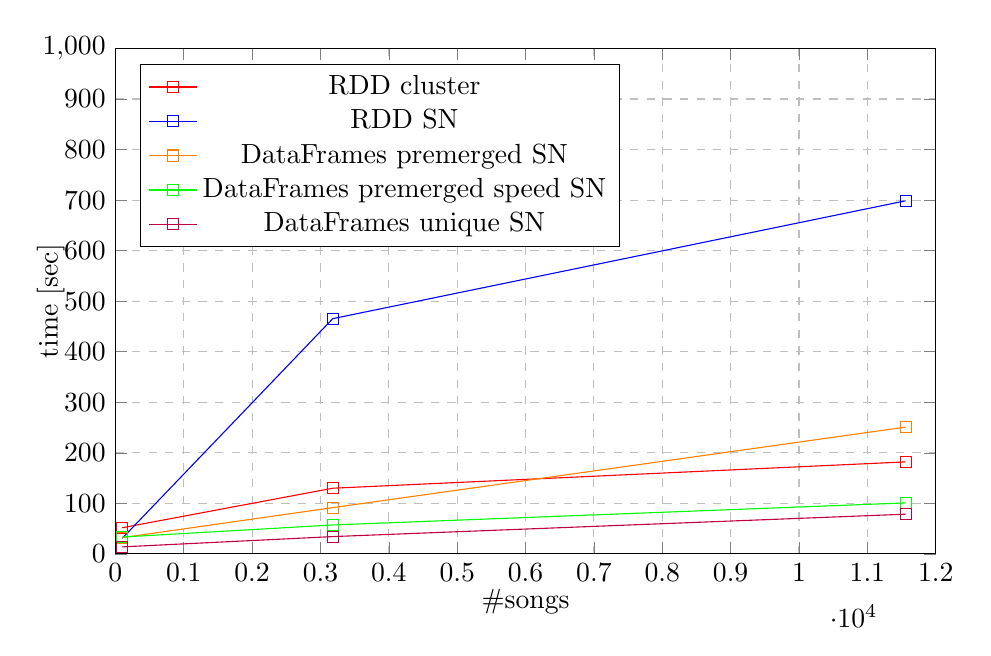
\begin{tikzpicture}
	\centering
	\begin{axis}[
	    %title={Performance of various toolkits},
		x label style={at={(axis description cs:0.5,-0.05)},anchor=north},
		y label style={at={(axis description cs:-0.05,.5)},rotate=0,anchor=south},
	    xlabel={\#songs},
	    ylabel={time [sec]},
	    xmin=0, xmax=12000,
	    ymin=0, ymax=1000,
	    xtick={0,1000,2000,3000,4000,5000,6000,7000,8000,9000,10000,11000,12000},
	    ytick={0,100,200,300,400,500,600,700,800,900,1000},
	    legend pos=north west,
	    ymajorgrids=true,
	    grid style=dashed,
	    height=8cm,
	    width=12cm,
	    grid=major,
	]
	\addplot[
		color=red,
		mark=square,
		]
		coordinates {
	    (100,51.736)(3180,129.940)(11560,182.035)
		};
		\addlegendentry{RDD cluster}
	\addplot[
	    color=blue,
	    mark=square,
	    ]
	    coordinates {
	    (100,30.770)(3180,465.445)(11560,698.657)
	    };
	    \addlegendentry{RDD SN}
	\addplot[
	    color=orange,
	    mark=square,
	    ]
	    coordinates {
	    (100,32.087)(3180,91.477)(11560,250.854)
	    };
	    \addlegendentry{DataFrames premerged SN}
	  
	\addplot[
	    color=green,
	    mark=square,
	    ]
	    coordinates {
	    (100,33.351)(3180,57.230)(11560,100.884)
	    };
	    \addlegendentry{DataFrames premerged speed SN}

	\addplot[
	    color=purple,
	    mark=square,
	    ]
	    coordinates {
	    (100,13.874)(3180,34.232)(11560,78.566)
	    };
	    \addlegendentry{DataFrames unique SN}	    
	\end{axis}
	\end{tikzpicture}
	\caption{Performance of various spark algorithms (MFCC Euc, Notes, RP)}
	\label{perfspark}
\end{figure}
\FloatBarrier


\subsubsection{min and max value aggregation}

\textit{\textbf{Why? Scaling of distances between 0 to 1 interval to combine different distances\\}}

\subsection{possible performance improvements}

\textit{\textbf{Pre- merge feature sets, broadcast comparator, descending importance pre-filtering\\}}
\\
\textit{\textbf{statistic normalization of similarities\\}}
\ \\
\textit{\textbf{Filter and refine after statistic normalization, drop all below mean\\}}
\ \\
\textit{\textbf{\underline{Is there a better way to cross-correlate???}\\}}
\ \\

\subsection{Descending Importance Filter and Refine}

\textit{\textbf{\underline{Make usage of caching from spark!}\\}}
\ \\

\textit{\textbf{\underline{order of operations is important -> für elise chroma first actually better in cover song recognition}\\}}
\ \\

\subsection{Other alternatives}

\subsubsection{Alternating Least Squares}

\subsubsection{TF-IDF weights}

\subsubsection{DIMSUM all-pairs similarity}